\section{Semiconductors}

\subsection{Conduction in semiconductors}
A uniform electric field $E_x$ is applied, which leads to a linearly decreasing potential
\begin{equation}
    \frac{dV}{dx} = -E_x
\end{equation}

%TODO: add graphic

This leads to a current density of
\begin{equation}
    J = e n v_{de} + e p v_{dh}
\end{equation}
where the drift velocities and mobilities for electrons and holes are
\begin{align*}
    v_{de} &= \mu_e E_x & \mu_e &= \frac{e \tau_e}{m_e^*} \\
    v_{dh} &= \mu_h E_x & \mu_h &= \frac{e \tau_h}{m_h^*}
\end{align*}
This leads to the conductivity
\begin{equation}
    \sigma = e n \mu_e + e p \mu_h
\end{equation}

\subsection{Electron and hole concentrations}
\begin{figure}[ht!]
    \centering
    %TODO: draw pic in tikz
    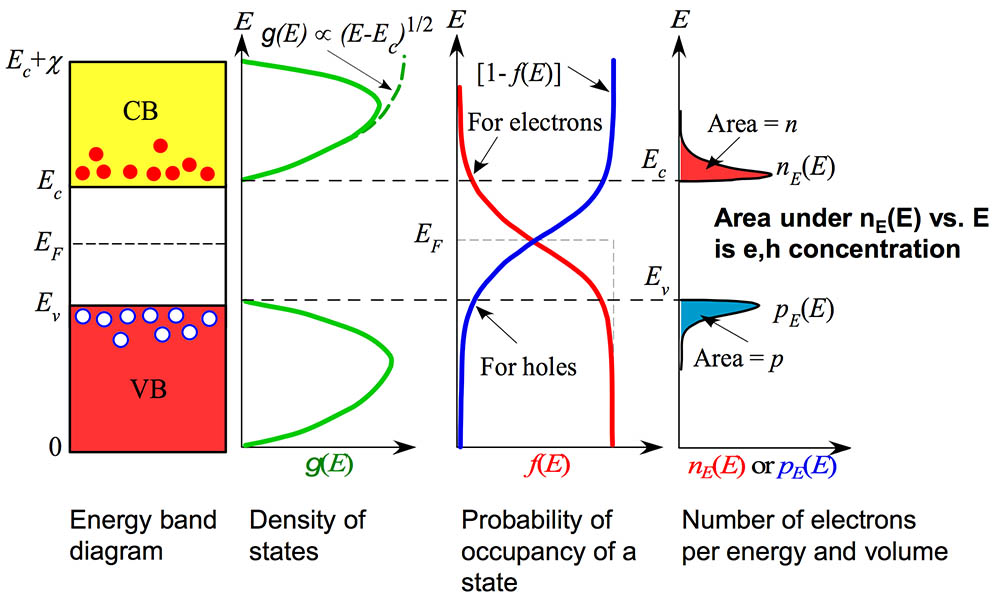
\includegraphics[width=0.6\linewidth]{images/semicond_elec_hole_concentration.jpg}
\end{figure}

The electron concentration $n$ and the hole concentration $p$ are calculated by
\begin{align}
    n &= N_C \cdot e^{-\frac{E_C-E_F}{k T}} && \text{with} & N_C &= 2 \left( \frac{2 \pi m_e^* k T}{h^2} \right)^{3/2} \\
    p &= N_V \cdot e^{-\frac{E_C-E_F}{k T}} && \text{with} & N_V &= 2 \left( \frac{2 \pi m_h^* k T}{h^2} \right)^{3/2}
\end{align}
where $N_C$ and $N_V$ are the effective densities of states at the CB edge and at the VB edge.

The mass action law states that
\begin{equation}
    n p = n_i^2 = N_C N_V \cdot e^{-\frac{E_C-E_V}{k T}} = N_C N_V \cdot e^{-\frac{E_G}{k T}}
\end{equation}
where $n_i$ is the electron and hole concentration in an intrinsic semiconductor.

\begin{table}[hbp!]
    \centering
    \begin{tabular}{lll}
        $n = p$ & $\Rightarrow$ & intrinsic semiconductor \\
        $n > p$ & $\Rightarrow$ & n-type semiconductor \\
        $p > n$ & $\Rightarrow$ & p-type semiconductor \\
    \end{tabular}
\end{table}

The Fermi energy in an intrinsic semiconductor is
\begin{align}
    E_{Fi} &= E_V + \frac{1}{2} E_g - \frac{1}{2} k T \ln \frac{N_C}{N_V} \\
    &= E_V + \frac{1}{2} E_g - \frac{3}{4} k T \ln \frac{m_e^*}{m_h^*} \\
    &= E_V + \frac{1}{2} E_g && \text{if} & m_e^*=m_h^* \:,\: N_C = N_V
\end{align}

%TODO: add image from 5.14
As $np = n_i^2$ must always be fulfilled,
\begin{align*}
    n \uparrow \;\Leftrightarrow\; E_F \uparrow && p \uparrow \;\Leftrightarrow\; E_F \downarrow
\end{align*}

\begin{figure}[htbp]
    \centering
    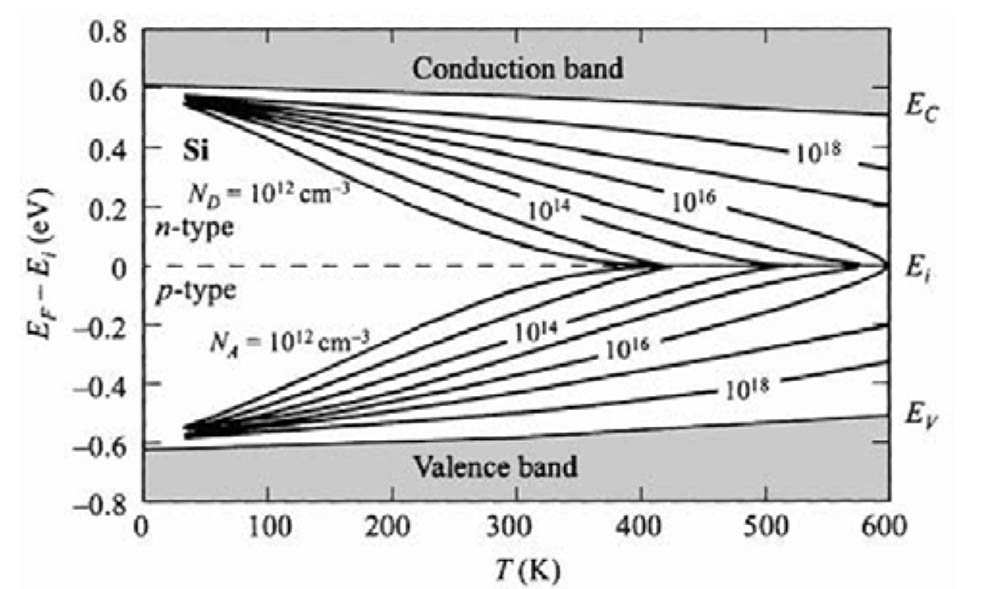
\includegraphics[width=0.6\linewidth]{images/semiconductors_fermi_energies.jpg}
    \caption{Fermi energy in silicon as a function of temperature and impurity concentration}
\end{figure}